\section{Lec 13}
This lecture is about establishing if spacetime is curved or not. We already attempt at this but failed:
\begin{itemize}
\item metric depends on the curvature
\item $\Gamma ^{\alpha }_{\beta \gamma } = 0$
\end{itemize}
Today we will develop an actual way to determine curvature of spacetime independently on coordinates chosen. This way is the \emph{Riemann Tensor.}\par

\subsubsection{Quick recall on LIC}
Local Inertial coordinates. Given a generic spacetime with generic coordinates system $x^{\mu }$ and metric tensor $g_{\mu \nu }$, for a given spacetime point \emph{P} we can find LIC $x^{\hat{\mu }}$. \par
So LIC at \emph{P} 
\begin{equation}
g_{\hat{\mu }\hat{\nu }} \left( P \right) = \eta _{\hat{\mu }\hat{\nu }}	
\end{equation}
obviously this is valid only in \emph{P}. Also $\partial_{\hat{\rho }} g_{\hat{\mu }\hat{\nu }} \left( P \right) = 0$

\subsubsection{Exponential Map}

Geodesics provide a convenient way of mapping the tangent space $T_{P}$ of a point $P$ to a region of the manifold that contains \emph{P}, called the \textbf{exponential map}. This map defines a set of coordinates for this region that are automatically the LIC, local inertial coordinates. \par
These is only one geodesic such that 
\[
x^{\mu }\left( \lambda = 0 \right) \to P
\]
Given a vector $k \in T_{P}$, it defines a unique geodesic passing through it, for which \emph{k} is the tangent vector at $P$, and $\lambda \left( P \right) = 0$:
\[
\frac{d x^{\mu }}{d \lambda } \left( \lambda =0 \right) \to k
\]
The uniqueness is given from the fact that the geodesic equation is a second order differential equation, and specifying the initial data in the form as above determines a solution.\par
So the exponential map at \emph{P}, so given a point in spacetime  
\begin{equation}
exp_{P} : T_{P} \to M
\end{equation}
is a map from the tangent space to a point on the manifold \emph{M}. And is defined as
\begin{equation}
exp_{P}\left( k \right) = x^{\mu }\left( \lambda =1 \right) \to Q
\end{equation}

The exponential map is invertible.

\tikzset{every picture/.style={line width=0.5pt}} %set default line width to 0.75pt
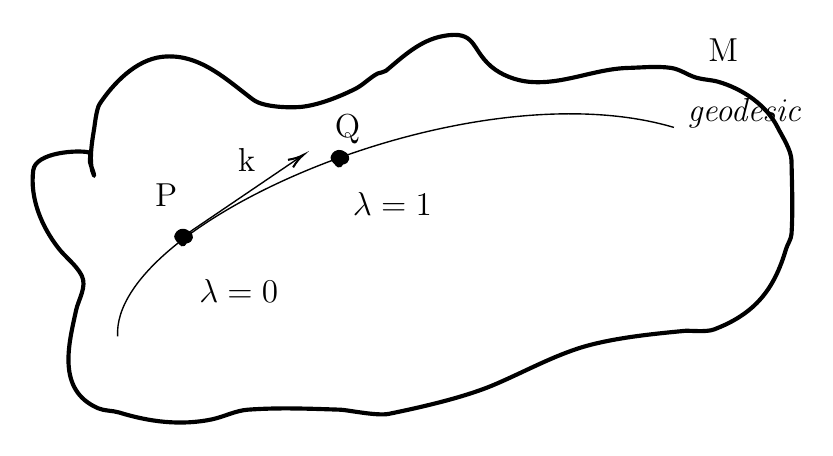
\begin{tikzpicture}[x=0.5pt,y=0.5pt,yscale=-1,xscale=1]
%Shape: Free Drawing [id:dp1885039918119823]
\draw  [line width=1.5] [line join = round][line cap = round] (93,148) .. controls (88.57,139.13) and (91.56,122.99) .. (93,114) .. controls (93.57,110.41) and (94.75,99.38) .. (97,96) .. controls (106.7,81.45) and (122.85,64.21) .. (142,62) .. controls (168.6,58.93) and (188.34,78.26) .. (208,93) .. controls (215.69,98.77) and (236.6,98.96) .. (244,98) .. controls (256.57,96.38) and (271,90.5) .. (282,85) .. controls (287.4,82.3) and (292.6,76.7) .. (298,74) .. controls (300.31,72.84) and (302.08,73.6) .. (304,72) .. controls (316.22,61.81) and (328.41,50.11) .. (345,47) .. controls (369.5,42.41) and (364.91,56.06) .. (380,69) .. controls (387.1,75.09) and (397.7,79.1) .. (407,80) .. controls (431.71,82.39) and (454.53,70.64) .. (479,70) .. controls (489.33,69.73) and (499.77,68.54) .. (510,70) .. controls (516.37,70.91) and (521.84,75.13) .. (528,77) .. controls (532.78,78.45) and (539.06,78.59) .. (544,80) .. controls (561.7,85.06) and (579,97) .. (587,113) .. controls (590.18,119.36) and (596.86,129.28) .. (597,137) .. controls (597.31,154.66) and (598.1,172.37) .. (597,190) .. controls (596.76,193.89) and (594.1,197.26) .. (593,201) .. controls (584.5,229.91) and (570.82,247.64) .. (541,259) .. controls (535.37,261.15) and (523.28,259.68) .. (520,260) .. controls (496.26,262.28) and (465.07,265.31) .. (442,273) .. controls (421.23,279.92) and (402.26,290.4) .. (382,299) .. controls (359.32,308.62) and (326.37,315.81) .. (306,320) .. controls (297.59,321.73) and (276.09,317.17) .. (271,317) .. controls (248.68,316.26) and (226.27,315.32) .. (204,317) .. controls (195.05,317.67) and (186.79,322.19) .. (178,324) .. controls (155.17,328.7) and (132.76,325.7) .. (111,319) .. controls (106.13,317.5) and (100.69,318.01) .. (96,316) .. controls (65.28,302.84) and (74.89,268.85) .. (80,245) .. controls (81.6,237.53) and (88.06,227.88) .. (84,220) .. controls (79.99,212.22) and (72.33,206.94) .. (67,200) .. controls (54.86,184.22) and (46.48,164.14) .. (49,144) .. controls (50.66,130.76) and (81.55,129.25) .. (89,131) .. controls (91.29,131.54) and (89.54,135.69) .. (90,138) .. controls (90.71,141.55) and (93,145.45) .. (93,148) -- cycle ;
%Curve Lines [id:da0957475647721604]
\draw    (110,264) .. controls (105,182) and (364,69) .. (512,113) ;
%Shape: Free Drawing [id:dp8414574325851908]
\draw  [line width=3] [line join = round][line cap = round] (157,196) .. controls (157,194.11) and (151.61,192.72) .. (155,190) .. controls (158.81,186.95) and (165.52,194) .. (158,194) ;
%Shape: Free Drawing [id:dp29626645456634426]
\draw  [line width=3] [line join = round][line cap = round] (270,139) .. controls (270,137.11) and (264.61,135.72) .. (268,133) .. controls (271.81,129.95) and (278.52,137) .. (271,137) ;
%Straight Lines [id:da5664923779397616]
\draw    (157,192) -- (242.34,134.12) ;
\draw [shift={(244,133)}, rotate = 145.86] [color={rgb, 255:red, 0; green, 0; blue, 0 }  ][line width=0.75]    (10.93,-3.29) .. controls (6.95,-1.4) and (3.31,-0.3) .. (0,0) .. controls (3.31,0.3) and (6.95,1.4) .. (10.93,3.29)   ;

% Text Node
\draw (535,47) node [anchor=north west][inner sep=0.75pt]   [align=left] {{\large M}};
% Text Node
\draw (135,152) node [anchor=north west][inner sep=0.75pt]   [align=left] {{\large P}};
% Text Node
\draw (265,102) node [anchor=north west][inner sep=0.75pt]   [align=left] {{\large Q}};
% Text Node
\draw (195,126) node [anchor=north west][inner sep=0.75pt]   [align=left] {{\large k}};
% Text Node
\draw (167,221) node [anchor=north west][inner sep=0.75pt]   [align=left] {\large $\lambda = 0$};
% Text Node
\draw (278,158) node [anchor=north west][inner sep=0.75pt]   [align=left] {\large $\lambda = 1$};
% Text Node
\draw (520,90) node [anchor=north west][inner sep=0.75pt]   [align=left] {\large \emph{geodesic}};
\end{tikzpicture}

\subsection{Riemann Normal Coordinates}
Given a generic $g_{\mu \nu }$ and a point \emph{P}, first I can find vectors $\hat{e}_{\left( \hat{\mu } \right)}$, (where the hat on the \emph{e} means that it is a basis vector and the hat on the index is means that is of inertial coordinates.)\par
Those are requirements to 
\[
g_{\hat{\mu }\hat{\nu }} =  g\left( \hat{e}_{\left( \hat{\mu } \right)}, \hat{e}_{\left( \hat{\nu } \right)} \right) = \eta _{\hat{\mu }\hat{\nu }}
\]
Where the \emph{g( , )} denotes the metric thought as a multilinear map from $T_{P} \times T_{P} \to \mathbb{R}$. This is easy because starting with any set of components for $g_{\mu \nu }$ we can always diagonalize this matrix and rescale the basis vectors to satisfy the above relation.\par
Now we want to find a coordinates system and to do that we will use the exponential map.
Let's define coordinates 
\begin{gather*}
x_{P} = 0 \\
x_{Q} = x^{\hat{\mu }}_{Q} \hat{e}_{\left( \hat{\mu } \right)} = k^{\hat{\mu }} \hat{e}_{\left( \hat{\mu } \right)}
\end{gather*}
where $x^{\hat{\mu }}_{Q}$ is the inverse of \emph{exp\textsubscript{P}}, \emph{x\textsubscript{Q}} is the position vector and it is represented as a linear combination of basis vectors.\par
So, RNC are $x_{Q } = k^{\mu } \hat{e}_{\left( \hat{\mu } \right)}$, and a particular property is that in this coordinates system 
\[
x^{\hat{\mu }}\left( \lambda  \right) = \lambda k^{\hat{\mu }}
\]
is a geodesic, only in these coordinates.
\subsubsection{More in deep explanation}
Now, I understand that if this is the first time approaching this it's kinda difficult to get the point. 
The part that makes the exponential map useful is that it's hard to find a coordinates system $x^{\hat{\mu }}$ for which the basis vectors $\{ \hat{e}_{\left( h\mu  \right)}\}$ are made of $\hat{e}_{\left( \hat{\mu } \right)} = \partial_{\hat{\mu } }$m and such that the first partial derivatives of $g_{\hat{\mu }\hat{\nu }}$ vanish. But the exponential map achieves that automatically. For any point \emph{Q} sufficiently close to \emph{P}, there is a unique geodesic path connecting \emph{P} to \emph{Q}, and a unique parametrization $\lambda $. At \emph{P} the tangent vector can be written as a linear combination of our basis vectors $k = k^{\hat{\mu }} \hat{e}_{\left( \hat{\mu } \right)}$. Then we define $x^{\hat{\mu }}$ to be these components $x^{\hat{\mu }}\left( Q \right) = k^{\hat{\mu }}$

\subsubsection{Check on RNC}
We want to verify that RNC satisfy $\partial_{\hat{\rho }} g_{\hat{\mu }\hat{\nu }}\left( P \right) = 0$. Noting that a ray  in the tangent space gets mapped to a geodesic by the exponential map, leads to see that in RNC a curve $x^{\hat{\mu }}\left( \lambda  \right)$ of the form
\[
x^{\hat{\mu }} \left( \lambda  \right) = \lambda k^{\hat{\mu }}
\]
will solve the geodesic equation.  Plugging this inside gives
\begin{equation}
\frac{d ^{2} x^{\hat{\mu }}}{d \lambda ^{2}} + \Gamma ^{\hat{\mu }}_{\hat{\alpha }\hat{\beta }} \frac{d x^{\hat{\alpha }}}{d \lambda }\frac{d x^{\hat{\beta }}}{d \lambda } = 0
\end{equation}
where the second derivative is null, and the other two partial derivatives correspond to $k^{\hat{\alpha }}, k^{\hat{\beta }}$. So we are left with
\begin{equation}
\Gamma ^{\hat{\mu }}_{\hat{\alpha }\hat{\beta }} k^{\hat{\alpha }}k^{\hat{\beta }} = 0, \forall k
\end{equation}
and since it true for every \emph{k}
\[
\Gamma ^{\hat{\mu }}_{\hat{\alpha }\hat{\beta }} \left( P \right) = 0
\]
Now we apply the metric compatibility
\begin{equation}
\nabla _{\hat{\rho }} \left( g_{\hat{\mu }\hat{\nu }} \right) = \partial_{\hat{\rho }} g_{\hat{\mu }\hat{\nu }} - \Gamma - \Gamma 
\end{equation}
And each term is equal to zero. RNCs makes the LICs.

\subsection{Riemann Curvature Tensor}

As we already discussed, parallel transport of a vector around a closed loop in a curved space will result in a different vector than the one we started with. The transformation depends on the total curvature enclosed by the loop. \par
Since spacetime looks flat locally, if we define a loop made by two infinitesimal vectors $A^{\mu }$ and $B^{\nu }$ we can  perform parallel transport on a vector $V^{\mu }$ by moving it anti-clockwise.


\tikzset{every picture/.style={line width=0.5pt}} %set default line width to 0.75pt      
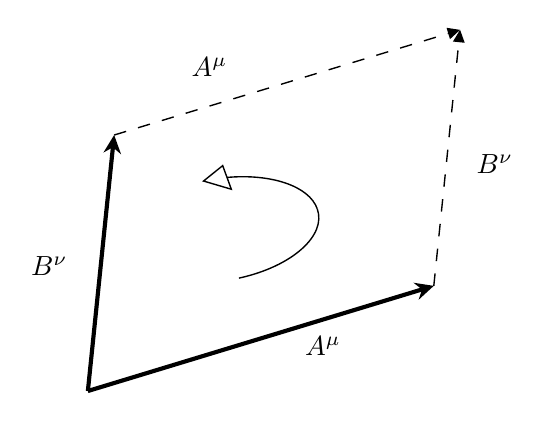
\begin{tikzpicture}[x=0.5pt,y=0.5pt,yscale=-1,xscale=1]
%uncomment if require: \path (0,300); %set diagram left start at 0, and has height of 300

%Straight Lines [id:da4139814907991093] 
\draw [line width=1.5]    (215,277) -- (461.17,202.16) ;
\draw [shift={(465,201)}, rotate = 163.09] [fill={rgb, 255:red, 0; green, 0; blue, 0 }  ][line width=0.08]  [draw opacity=0] (13.4,-6.43) -- (0,0) -- (13.4,6.44) -- (8.9,0) -- cycle    ;
%Straight Lines [id:da37994344236993594] 
\draw [line width=1.5]    (215,277) -- (233.59,95.98) ;
\draw [shift={(234,92)}, rotate = 95.86] [fill={rgb, 255:red, 0; green, 0; blue, 0 }  ][line width=0.08]  [draw opacity=0] (13.4,-6.43) -- (0,0) -- (13.4,6.44) -- (8.9,0) -- cycle    ;
%Straight Lines [id:da11748394321022726] 
\draw  [dash pattern={on 4.5pt off 4.5pt}]  (465,201) -- (483.69,18.98) ;
\draw [shift={(484,16)}, rotate = 95.86] [fill={rgb, 255:red, 0; green, 0; blue, 0 }  ][line width=0.08]  [draw opacity=0] (8.93,-4.29) -- (0,0) -- (8.93,4.29) -- cycle    ;
%Straight Lines [id:da04954610847070795] 
\draw  [dash pattern={on 4.5pt off 4.5pt}]  (234,92) -- (481.13,16.87) ;
\draw [shift={(484,16)}, rotate = 163.09] [fill={rgb, 255:red, 0; green, 0; blue, 0 }  ][line width=0.08]  [draw opacity=0] (8.93,-4.29) -- (0,0) -- (8.93,4.29) -- cycle    ;
%Curve Right Arrow [id:dp34474738978659925] 
\draw  [fill={rgb, 255:red, 255; green, 255; blue, 255 }  ,fill opacity=1 ] (380.74,145.2) .. controls (387.81,164.58) and (362.48,187.06) .. (324.16,195.41) -- (324.16,195.41) .. controls (362.48,187.06) and (387.81,164.58) .. (380.74,145.2) -- cycle ;\draw  [fill={rgb, 255:red, 255; green, 255; blue, 255 }  ,fill opacity=1 ] (380.74,145.2) .. controls (374.73,128.72) and (347.22,119.8) .. (315.56,122.64) -- (318.67,131.17) -- (298.58,125.25) -- (312.44,114.11) -- (315.56,122.64) .. controls (347.22,119.8) and (374.73,128.72) .. (380.74,145.2) -- cycle ;

% Text Node
\draw (172,178) node [anchor=north west][inner sep=0.75pt]   [align=left] { $B^{\nu }$ };
% Text Node
\draw (370,236) node [anchor=north west][inner sep=0.75pt]   [align=left] { $A^{\mu }$};
% Text Node
\draw (494,104) node [anchor=north west][inner sep=0.75pt]   [align=left] { $B^{\nu }$};
% Text Node
\draw (288,34) node [anchor=north west][inner sep=0.75pt]   [align=left] { $A^{\mu }$};
\end{tikzpicture}
\bigskip

As we know the action of parallel transport is independent on the coordinates, so there should be a tensor that quantifies the change of the vector, so with an upper and a lower index. Depending also on vectors \textbf{A} and \textbf{B}, there are two additional lower indices. And this tensor must be anti-symmetric since we can walk the loop in the opposite direction, and the outcome would be the inverse. So we should get something like this
\begin{equation}
\delta V^{\mu } = R^{\mu }_{\alpha \beta \gamma }A^{\alpha }B^{\beta }V^{\gamma}
\end{equation}
As decided above this tensor should be anti-symmetric on the \emph{last two indices}.
\[
R^{\mu }_{\alpha \beta \gamma } = - R^{\mu }_{\alpha \gamma  \beta }
\]
To compute what's inside the \textbf{R} tensor is kinda difficult so we take a related operation, the commutator of two covariant derivatives. \par
The relation between the two is because the covariant derivative of a tensor in a certain direction measures how much the tensor changes relative to what it would have been if it had been parallel transported, because the covariant derivative of a tensor in a direction along which is parallel transported is null. The commutator of two covariant derivatives measures the difference between parallel transporting the tensor first one way and then the other, and viceversa.\bigskip


\tikzset{every picture/.style={line width=0.5pt}} %set default line width to 0.75pt       
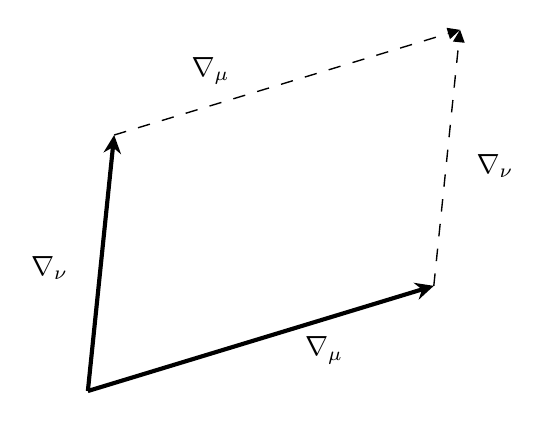
\begin{tikzpicture}[x=0.5pt,y=0.5pt,yscale=-1,xscale=1]
%uncomment if require: \path (0,300); %set diagram left start at 0, and has height of 300

%Straight Lines [id:da4139814907991093] 
\draw [line width=1.5]    (215,277) -- (461.17,202.16) ;
\draw [shift={(465,201)}, rotate = 163.09] [fill={rgb, 255:red, 0; green, 0; blue, 0 }  ][line width=0.08]  [draw opacity=0] (13.4,-6.43) -- (0,0) -- (13.4,6.44) -- (8.9,0) -- cycle    ;
%Straight Lines [id:da37994344236993594] 
\draw [line width=1.5]    (215,277) -- (233.59,95.98) ;
\draw [shift={(234,92)}, rotate = 95.86] [fill={rgb, 255:red, 0; green, 0; blue, 0 }  ][line width=0.08]  [draw opacity=0] (13.4,-6.43) -- (0,0) -- (13.4,6.44) -- (8.9,0) -- cycle    ;
%Straight Lines [id:da11748394321022726] 
\draw  [dash pattern={on 4.5pt off 4.5pt}]  (465,201) -- (483.69,18.98) ;
\draw [shift={(484,16)}, rotate = 95.86] [fill={rgb, 255:red, 0; green, 0; blue, 0 }  ][line width=0.08]  [draw opacity=0] (8.93,-4.29) -- (0,0) -- (8.93,4.29) -- cycle    ;
%Straight Lines [id:da04954610847070795] 
\draw  [dash pattern={on 4.5pt off 4.5pt}]  (234,92) -- (481.13,16.87) ;
\draw [shift={(484,16)}, rotate = 163.09] [fill={rgb, 255:red, 0; green, 0; blue, 0 }  ][line width=0.08]  [draw opacity=0] (8.93,-4.29) -- (0,0) -- (8.93,4.29) -- cycle    ;

% Text Node
\draw (172,178) node [anchor=north west][inner sep=0.75pt]   [align=left] { $\nabla _{\nu }$};
% Text Node
\draw (370,236) node [anchor=north west][inner sep=0.75pt]   [align=left] { $\nabla _{\mu }$};
% Text Node
\draw (494,104) node [anchor=north west][inner sep=0.75pt]   [align=left] { $\nabla _{\nu }$};
% Text Node
\draw (288,34) node [anchor=north west][inner sep=0.75pt]   [align=left] { $\nabla _{\mu }$};
\end{tikzpicture}
\bigskip

We could do the computation with a scalar but
\begin{equation}
	[\nabla _{\mu }, \nabla _{\nu }] \phi = \nabla _{\mu}\left( \nabla _{\nu }\phi  \right) -\nabla _{\nu }\left( \nabla _{\mu }\phi  \right) = \partial_{\mu }\left( \partial_{\nu }\phi  \right) - \partial_{\nu }\left( \partial_{\mu }\phi  \right) = 0
\end{equation}
Not only is equal to zero, but it's trivially zero.\par
So we will use a vector
\begin{gather*}
	[\nabla _{\mu },\nabla _{\nu }] V^{\rho } = \nabla _{\mu }\left( \nabla _{\nu }V^{\rho } \right) - \nabla_{\nu }\left( \nabla _{\mu }V^{\rho } \right)	 \\
	\text{ now we take just one of the terms } \\
	\nabla _{\mu }\left( \nabla _{\nu } V^{\rho } \right) = \partial_{\mu } \left( \nabla _{\nu } V^{\rho } \right) + \Gamma ^{\rho }_{\mu \beta } \nabla _{\nu }V^{\beta } - \Gamma ^{\beta }_{\mu \nu } \nabla _{\beta } V^{\rho } \\
	\text{ again, we take the first term of the second part } \\
	\partial_{\mu }\left( \partial_{\nu }V^{\rho } + \Gamma ^{\rho }_{\nu \alpha } V^{\alpha } \right) + \Gamma ^{\rho }_{\mu \beta } \left( \partial_{\nu }V^{\beta } + \Gamma ^{\beta}_{\nu \alpha } V^{\alpha } \right) - \Gamma ^{\beta }_{\mu \nu } \nabla _{\beta }V^{\rho } \\
	\partial_{\mu }\partial_{\nu }V^{\rho } + \left( \partial_{\mu } \Gamma ^{\rho }_{\nu \alpha } \right)V^{\alpha } + \Gamma ^{\rho }_{\nu \alpha } \partial_{\mu }V^{\alpha } + \Gamma ^{\rho }_{\mu \beta } \partial_{\nu }V^{\beta } + \Gamma ^{\rho }_{\mu \beta }\Gamma ^{\beta }_{\nu \alpha } V^{\alpha }- \Gamma ^{\beta }_{\mu \nu }\nabla _{\beta} V^{\rho }
\end{gather*}
Now, let's look at this last row for some simplifications.
\begin{itemize}
\item The first term is symmetric in $\mu , \nu $.
\item The sum of the third and the fourth is symmetric in $\mu , \nu $ if we swap the dummy index $\beta \to \alpha $.
\item The last term is symmetric but only with \emph{zero torsion,}
\end{itemize}
The terms that are symmetric vanish since we are using the operator of anti-symmetry. So we are left, with
\begin{equation}
	[\nabla _{\mu }, \nabla _{\nu }]V^{\rho } = \left( \partial_{\mu }\Gamma ^{\rho }_{\nu \alpha } - \partial_{\nu }\Gamma ^{\rho }_{\mu \alpha } \right)V^{\alpha } + \left( \Gamma ^{\rho }_{\mu \beta } \Gamma ^{\beta }_{\nu \alpha } - \Gamma ^{\rho }_{\nu \beta }\Gamma ^{\beta }_{\mu \alpha } \right)V^{\alpha } - \left( \Gamma ^{\beta }_{\mu \nu } - \Gamma ^{\beta }_{\nu \mu } \right)\nabla _{\beta }V^{\rho }
\end{equation}
This last piece has equivalent to the \emph{torsion} that is
\[
T^{\beta }_{\mu \nu }\nabla _{\beta }V^{\rho }
\]
but since we work with torsion free connections, it's zero. We are left with
\begin{equation}
	[\nabla _{\mu }, \nabla _{\nu }]V^{\rho } = [\partial_{\mu }\Gamma ^{\rho }_{\nu \alpha } - \partial_{\nu }\Gamma ^{\rho }_{\mu \alpha } + \Gamma  ^{\rho }_{\mu  \beta }\Gamma  ^{ \beta }_{\nu  \alpha } - \Gamma ^{\rho }_{\nu \beta }\Gamma ^{\beta }_{\mu \alpha }] V^{\alpha }
\end{equation}
And this, can be written as 
\begin{equation}
	[\nabla _{\mu }, \nabla _{\nu }] V^{ \rho } = R^{\rho }_{\sigma \mu \nu } V^{\sigma }
\end{equation}
that is the Riemann Tensor.






